%% Produit par outils/generer_lecture.py — ne pas modifier à la main.
\begin{tabular*}{0.68\linewidth}{@{\extracolsep{\fill}}ccc@{}}

\includegraphics{l-cle-sol.cropped.pdf} &

\includegraphics{l-cle-fa.cropped.pdf} &

\includegraphics{l-cle-fa3.cropped.pdf} \\[2pt]
\small clé de sol & \small clé de fa & \small clé de fa \\
\small\color{mygray} sol3, 2\textsuperscript{e} ligne &
\small\color{mygray} fa2, 4\textsuperscript{e} ligne &
\small\color{mygray} fa2, 3\textsuperscript{e} ligne \\
\end{tabular*}
\\[10pt]
\begin{tabular*}{0.9\linewidth}{@{\extracolsep{\fill}}cccc@{}}
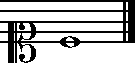
\includegraphics{l-cle-ut1.cropped.pdf} &
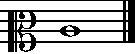
\includegraphics{l-cle-ut2.cropped.pdf} &

\includegraphics{l-cle-ut3.cropped.pdf} &

\includegraphics{l-cle-ut4.cropped.pdf} \\[2pt]
\small clé d'ut & \small clé d'ut & \small clé d'ut & \small clé d'ut \\
\small\color{mygray} do3, 1\textsuperscript{re} ligne &
\small\color{mygray} do3, 2\textsuperscript{e} ligne &
\small\color{mygray} do3, 3\textsuperscript{e} ligne &
\small\color{mygray} do3, 4\textsuperscript{e} ligne \\
\end{tabular*}
